\documentclass[varwidth=true, border=2pt]{standalone}

\usepackage{pgfplots}
\usepackage{tikz}
\usetikzlibrary{positioning}
\usetikzlibrary{decorations.text}
\usetikzlibrary{decorations.pathmorphing}

\begin{document}
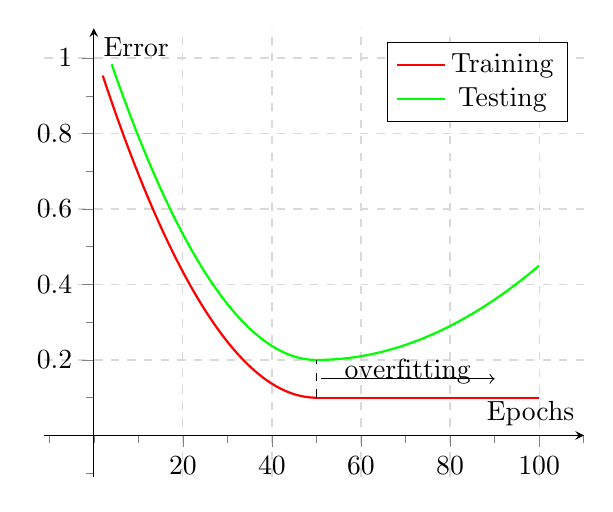
\begin{tikzpicture}
    \begin{axis}[
        legend pos=north east,
        axis x line=middle,
        axis y line=middle,
        grid = major,
        %width=9cm,
        %height=4.5cm,
        grid style={dashed, gray!30},
        xmin=-1,     % start the diagram at this x-coordinate
        xmax= 100,    % end   the diagram at this x-coordinate
        ymin=-0.01,     % start the diagram at this y-coordinate
        ymax= 0.98,   % end   the diagram at this y-coordinate
        axis background/.style={fill=white},
        xlabel=Epochs,
        ylabel=Error,
        %xticklabels={-2,-1.6,...,7},
        %yticklabels={-8,-7,...,8},
        tick align=outside,
        minor tick num=-3,
        enlargelimits=true,
        tension=0.08]
      \addplot[domain=2:50, red, thick,samples=200] {(x-50)^2/2700 + 0.1};
      \addplot[domain=4:50, green, thick,samples=200] {(x-50)^2/2700 + 0.2};

      \addplot[domain=50:100, red, thick,samples=200] {0.1};
      \addplot[domain=50:100, green, thick,samples=200] {(x-50)^2/10000 + 0.2};

      \draw[dashed] (axis cs:50,0.1) -- (axis cs:50,0.2);
      \draw[decoration={text along path, text={overfitting}, text align={center}}, decorate] (axis cs:51,0.15) -- (axis cs:90,0.15);
      \draw[->] (axis cs:51,0.15) -- (axis cs:90,0.15);

      \addlegendentry{Training}
      \addlegendentry{Testing}
    \end{axis}
\end{tikzpicture}
\end{document}
